\documentclass[11pt]{article}

\usepackage{float}
\usepackage{hyperref}
\usepackage{graphicx}
% formatting
\usepackage{verbatim}
\usepackage{moreverb}
\usepackage{minted}
\usepackage{parskip}
\usepackage{amsmath}
\usepackage[listings]{tcolorbox}
\usepackage{enumerate}
\let\verbatiminput=\verbatimtabinput
\def\verbatimtabsize{4\relax}

\newcommand{\RepoRootPath}{fpga\_labs\_fa19}

\tcbset{
texexp/.style={colframe=black, colback=lightgray!15,
         coltitle=white,
         fonttitle=\small\sffamily\bfseries, fontupper=\small, fontlower=\small},
     example/.style 2 args={texexp,
title={Question \thetcbcounter: #1},label={#2}},
}

\newtcolorbox{texexp}[1]{texexp}
\newtcolorbox[auto counter]{texexptitled}[3][]{%
example={#2}{#3},#1}

\setlength{\topmargin}{-0.5in}
\setlength{\textheight}{9in}
\setlength{\oddsidemargin}{0in}
\setlength{\evensidemargin}{0in}
\setlength{\textwidth}{6.5in}

% Useful macros

\newcommand{\note}[1]{{\bf [ NOTE: #1 ]}}
\newcommand{\fixme}[1]{{\bf [ FIXME: #1 ]}}
\newcommand{\wunits}[2]{\mbox{#1\,#2}}
\newcommand{\um}{\mbox{$\mu$m}}
\newcommand{\xum}[1]{\wunits{#1}{\um}}
\newcommand{\by}[2]{\mbox{#1$\times$#2}}
\newcommand{\byby}[3]{\mbox{#1$\times$#2$\times$#3}}


\newenvironment{tightlist}
{\begin{itemize}
 \setlength{\parsep}{0pt}
 \setlength{\itemsep}{-2pt}}
{\end{itemize}}

\newenvironment{titledtightlist}[1]
{\noindent
 ~~\textbf{#1}
 \begin{itemize}
 \setlength{\parsep}{0pt}
 \setlength{\itemsep}{-2pt}}
{\end{itemize}}

% Change spacing before and after section headers

\makeatletter
\renewcommand{\section}
{\@startsection {section}{1}{0pt}
 {-2ex}
 {1ex}
 {\bfseries\Large}}
\makeatother

\makeatletter
\renewcommand{\subsection}
{\@startsection {subsection}{1}{0pt}
 {-1ex}
 {0.5ex}
 {\bfseries\normalsize}}
\makeatother

% Reduce likelihood of a single line at the top/bottom of page

\clubpenalty=2000
\widowpenalty=2000

% Other commands and parameters

\pagestyle{myheadings}
\setlength{\parindent}{0in}
\setlength{\parskip}{10pt}

% Commands for register format figures.

\newcommand{\instbit}[1]{\mbox{\scriptsize #1}}
\newcommand{\instbitrange}[2]{\instbit{#1} \hfill \instbit{#2}}
\newcommand{\itwos}{I\textsuperscript{2}S}

\begin{document}

\def\PYZsq{\textquotesingle}
\title{\vspace{-0.4in}\Large \bf EECS 151/251A FPGA Lab Spring 2021\\
Lab 3:\\FPGA Memory Blocks, FSM Calculator\vspace{-0.1in}}

\author{Prof. John Wawrzynek \\
TAs: Sean Huang, Tan Nguyen \\ Department of Electrical Engineering and Computer Sciences\\
College of Engineering, University of California, Berkeley}
\date{}
\maketitle

\section{Before You Start This Lab}\label{sec:begin}
You should run \verb|git pull| in \verb|fpga_labs_sp21| to get the latest files for this lab.

Replace the following files with your code from Lab 2.
\begin{itemize}
  \item \verb|lab3/src/debouncer.v|
  \item \verb|lab3/src/synchronizer.v|
  \item \verb|lab3/src/edge_detector.v|
\end{itemize}

You should also review the lecture slides on Finite-State Machine. For additional resource, take a look at \href{http://inst.eecs.berkeley.edu/~eecs151/sp21/files/verilog/verilog\_fsm.pdf}{verilog\_fsm.pdf}

%In this lab, we cover FPGA memories and audio. We will learn to how to leverage the memory resource on FPGA for data storage. In addition, we will build circuits that play musical tones by implementing an I2S protocol to interface with an off-chip DAC (Digital-to-Analog) of Pmod I2S module. If you do not have a Pmod I2S module around when you start working on this lab, please notify a TA.

In this lab, we implement some designs using the FPGA Memory blocks. Way in the semester, the lectures will cover the Memory modules in details down to the transistor level. For the purpose of this lab, we would like to give you some overview of the memory modules since they are prevalent in digital design and enable us to build more interesting applications, and hopefully you will be able to connect with the lecture materials later.
%In digital design, it is important to know the timing information of the input and output pins of a hardware block in order to use it effectively.

\section{FPGA Memory Blocks}

Recall that in Lab 1, we explored different types of resources on our FPGA. Besides the LUTs and FFs for combinational and sequential logic implementation, our FPGA chip also offers Memory LUTs (from SLICEM) and Block RAMs for dense on-chip data storage. Some most recent Xilinx FPGA chips employ Ultra RAM blocks with even greater density. This brings many benefits as the read/write accesses to those memory blocks are fast and predictable (i.e., the number of cycles for read/write is known), unlike off-chip memory accesses. Note that an FPGA has no cache. You as a hardware designer will need to build your own datapath and control logic to manage memory accesses and storage on the FPGA. One benefit is that you can tailor this flexibility to your own application's memory requirement and access patterns to achieve much better performance than a traditional cache-based systems. The density of those memory blocks also reduces the register pressure when you need a large number of state elements in your design; you will see an example of that in one of the lab exercises. In the final project, the Memory blocks are utilized to implement the data storage modules for your processor, such as register file, instructional and data memory.

Take a look at the file \verb|lib/EECS151.v|. Besides the REGISTER modules, we have added some memory modules. What's different from the REGISTER modules is that we now have an address input pin for each memory module. Typically, a memory port refers to a set of signals {\texttt{clk} (clock), \texttt{addr} (address pin),  \texttt{wen} (write-enable), \texttt{d} (data input), \texttt{q} (data output) (and the optional \texttt{en} (enable) pin). In this lab, we deal with single-port memory blocks. As we will see in later labs, there are also dual-port memory modules.

Regarding timing characteristics. there are two types of memory blocks that we should pay attention for now: \textbf{Asynchronous Read and Synchronous Write} Memory, and \textbf{Synchronous Read and Synchronous Write} Memory. The synchronicity is with respect to the input clock signal. When write, both types write the data to their storages at the next clock edge (write takes one cycle). When read, asynchronous read data appears on the data output pin in the same cycle as the address pin applies/changes (read happens immediately), whereas synchronous read data is only available at the next clock edge (read takes one cycle)
An asychronous-read Memory block typically gets mapped to Distributed RAMs on an FPGA (Memory LUTs/LUTRAMs), while a synchronous-read Memory block is mapped to Block RAMs (BRAMs).
Both can also be utilized as ROM-style memory blocks for read-only data storage. Using ROMs also yields simpler control logic if you don't do any memory updates. Note that the typical logic LUTs from SLICEL can also be used to implement ROMs.

You can have a look at the timing diagram of an FPGA LUTRAM to understand how asynchronous read and synchronous write work (page 65, \href{http://www.xilinx.com/support/documentation/user_guides/ug474_7Series_CLB.pdf}{Xilinx 7-series Configurable Logic Block User Guide}). Note how a memory write is synchronous with the clock edge when \texttt{WE} is HIGH, and read is spontaneous.

\begin{center}
%\fbox{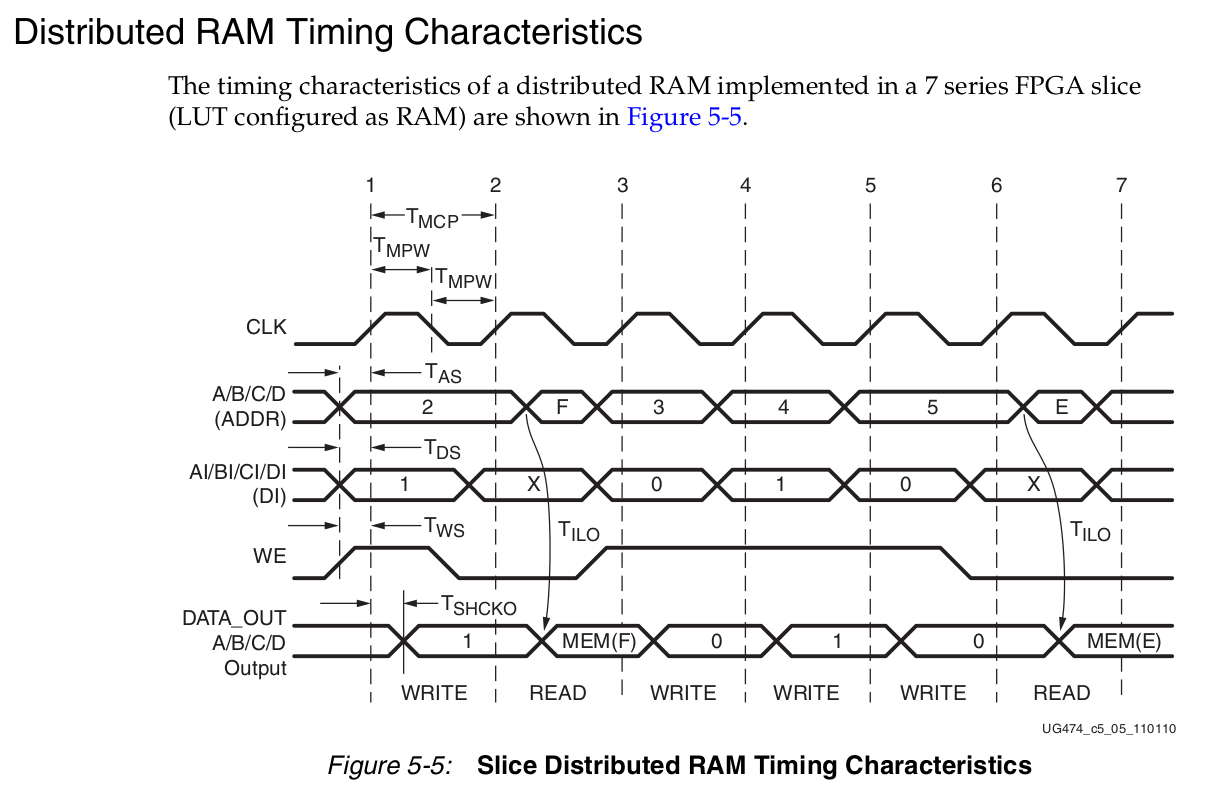
\includegraphics[width=0.7\textwidth]{figs/lutram_timing.png}}
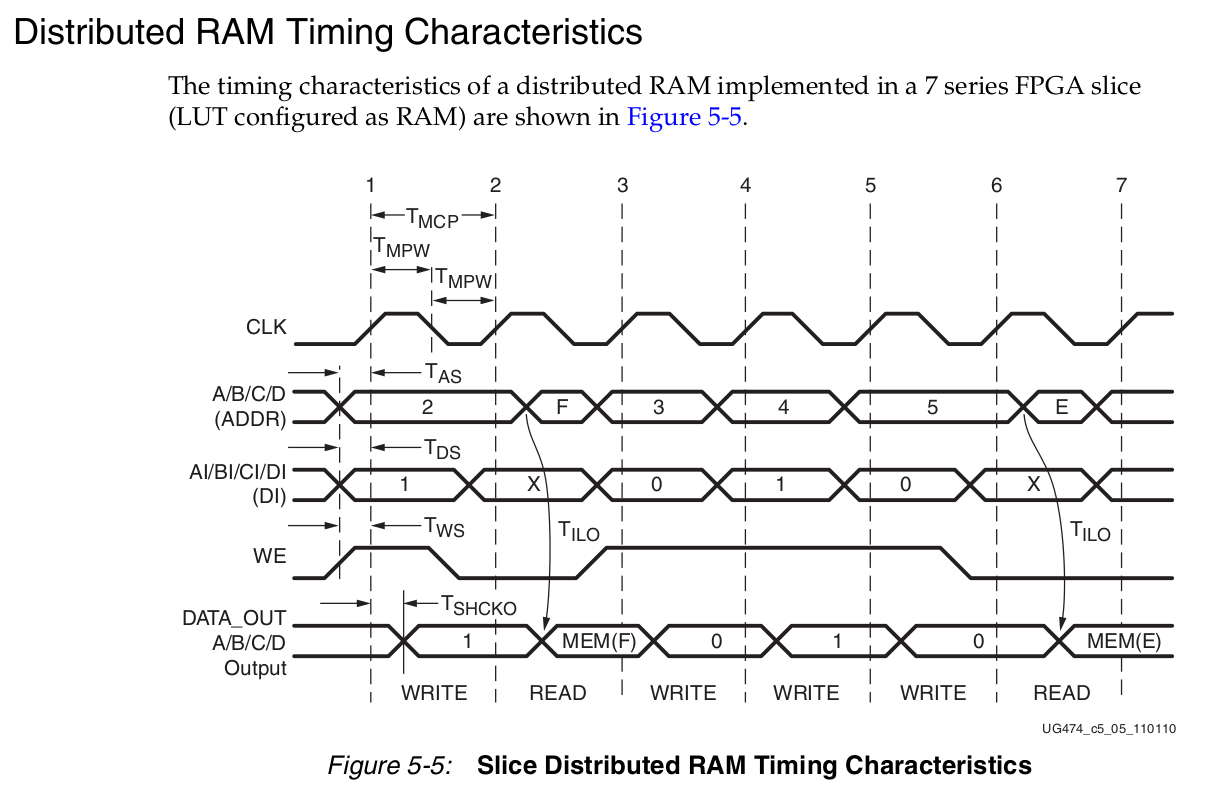
\includegraphics[width=0.7\textwidth]{figs/lutram_timing.png}
\end{center}

Since we are adopting the "No Register inference" policy in this semester, you won't be asked to code your own memory blocks in the lab exercises and the project. Rather, we will provide the memory templates for you as similar to the REGISTER modules in \verb|lib/EECS151.v|; they are guaranteed to be synthesized to memory blocks by Vivado correctly. However, for your learning, it is certainly important to be aware of how a piece of Verilog code gets synthesized to a memory block.
The memory are declared as an array of \verb|reg| nets as follows.

\begin{minted}[tabsize=2]{verilog}
(* ram_style = "block" *) reg [DWIDTH-1:0] mem [DEPTH-1:0];
\end{minted}

Depending on how you write your Verilog code that makes use of this \verb|reg|, the Synthesis tool will infer this \verb|reg| as either a bunch of separate registers or some form of dense memory block(s). Certain vendors adopt some specific coding styles or synthesis attributes that give hints to the tools to map your hardware nets to which FPGA resources. Here, the attribute \verb|ram_style = "block"| tells Vivado synthesis that we want to map this \verb|reg| to Block RAMs. Normally, we just let the tools to figure out what resources are best to use to create optimal designs. Sometimes the tool makes a decision based on the resource utilization of your designs and the availability of the resource on the target board. The tool also considers which resource to use to minimize the logic and interconnect delay. Most of the time, a hardware design just relies on the tool. Nonetheless, the tool also offers some synthesis attributes to give us the flexibility to force the tool to do what we want. Note that those attributes or coding styles may not apply from one vendor tool to another, so you should always consult the Synthesis user guide of your vendor tools.
If you are interested to learn more, you should definitely take a look at \href{https://www.xilinx.com/support/documentation/sw_manuals/xilinx2019_2/ug901-vivado-synthesis.pdf}{Vivado Synthesis Guide}, Chapter 2 and 4. Look at page 110 to see some examples of RAM HDL Coding techniques.

We can initialize the content of our memory blocks with the following Verilog constructs.

\begin{minted}[tabsize=2]{verilog}
initial begin
  if (MIF_HEX != "") begin
    $readmemh(MIF_HEX, mem);
  end
  else if (MIF_BIN != "") begin
    $readmemb(MIF_BIN, mem);
  end
end
\end{minted}

The Verilog code looks for a memory initialization file \verb|mif| to initialize the content of \verb|mem|. If the numeric data of the \verb|mif| file is in hex format, use \verb|$readmemh|, otherwise if it is in binary format, use \verb|$readmemb|. This works for both Bitstream Generation and Simulation too.
This method can be used to implement a ROM-style memory block. Here is a different method to create an asynchronous ROM or a look-up table.

\begin{minted}[tabsize=2]{verilog}
module rom (input [2:0] address, output reg [11:0] data);
  always @(*) begin
    case(address)
      3'd0: data = 12'h000;
      3'd1: data = 12'hFFF;
      3'd2: data = 12'hACD;
      3'd3: data = 12'h122;
      3'd4: data = 12'h347;
      3'd5: data = 12'h93A;
      3'd6: data = 12'h0AF;
      3'd7: data = 12'hC2B;
    endcase
  end
endmodule
\end{minted}

Note that you are free to use this method in your design file, since it does not use a sequential always block. This is useful if you just want to create a small look-up table. Other than that, for this and later labs, please use the memory modules declared in \verb|lib/EECS151.v| when you want to instantiate a memory block, just like the REGISTER policy. We'd like you to avoid writing explicit sequential logic with \verb|always @(posedge clk)| and non-blocking assignments in your design files.

\subsection{Questions: Understanding Your FPGA Memory blocks}\label{sec:Q1}
Skim the \href{http://www.xilinx.com/support/documentation/user_guides/ug474_7Series_CLB.pdf}{Xilinx 7-series CLB User Guide}, and \href{https://www.xilinx.com/support/documentation/user_guides/ug473_7Series_Memory_Resources.pdf}{Xilinx 7-Series Memory Resource} (pay attention to the Summary pages), and \href{https://www.xilinx.com/support/documentation/sw_manuals/xilinx2019_2/ug901-vivado-synthesis.pdf}{Vivado Synthesis Guide} (pages 117-123)
\begin{enumerate} 
\item Compared to a normal logic LUT from a SLICEL, what are some additional pins presented in a Memory LUT (LUTRAM) and what are they used for? What is a memory capacity of a single Memory LUT?
\item When looking at the datasheet of an FPGA device or resource utilization report, we often see that the BRAM resource is reported as a number of either 36Kb BRAMs or 18Kb BRAMs. How does a 36Kb-BRAM block differ from a 18Kb-BRAM block?
\item How are the Block RAMs laid out on an FPGA? Can you tell at least one advantage of such organization?
\item What is the difference between the \textit{WRITE FIRST} mode and the \textit{READ FIRST} mode of a BRAM? What is the mode of the Memory module \texttt{SYNC\_RAM} implemented in \verb|lib/EECS151.v|?
\end{enumerate}

Let's do some practice with the memory blocks.

\subsection{Design a Register File}

In this section, you will build a parameterized Register File module composed of REGISTER blocks. Our simple Register File module has a single port for read or writea {\texttt{clk}, \texttt{we}, \texttt{addr}, \texttt{din}, \texttt{dout}}. The address and data width are parameterizable. Refer to the following block diagram for the details.

\begin{center}
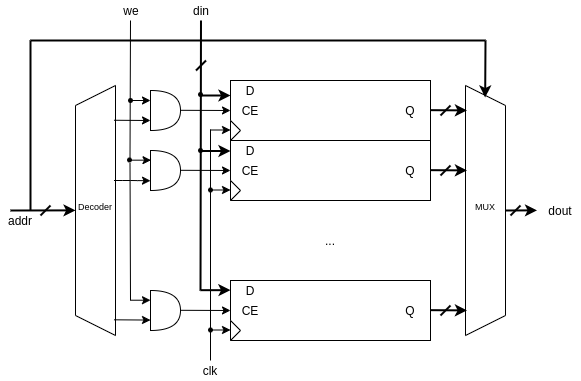
\includegraphics[width=0.7\textwidth]{figs/regfile.png}
\end{center}

Fill in the necessary logic in \verb|lab3/src/register_file.v| to implement your Register file. A testbench code has been provided for you: \verb|lab3/sim/register_file_tb.v| (please read the testbench code to understand what is being tested, and add your own tests if you see fit).

Once you pass the simulation, use \verb|lab3/src/z1top_register_file.v| as the top-level module to generate a bitstream to test your register file on the PYNQ. This circuit also requires the \textbf{button parser} logic that you implemented in \textbf{Lab 2}, so make sure you have the \verb|button_parser| module ready with your code. The circuit allows you to specify a location of the register file to store/load data. You will use the buttons to provide input location or data, and observe the results with the LEDs. Read the code carefully to understand how to use the buttons and switches to run it and what to expect. If you are unsure or spot any issues, please do not hesitate to talk to a TA.

If your register file implementation works on the board, good work! Note down the resource utilization in terms of LUTs and FFs (If you forget where to find the resource utilization report, check Lab 1. You can also find that information from the Vivado GUI). Next, modify your Register File implementation (\verb|lab3/src/register_file.v|) to use the \texttt{ASYNC\_RAM} module from \verb|lib/EECS151.v|, and run the tool again to produce a bitstream to test it on your board (make sure you pass the simulation first!). Also record the resource utilization in this case.

\subsection{Questions: REGISTERs vs. Memory Blocks}\label{sec:Q2}
\begin{enumerate}
\item Compare the resource utilization between the two implementations. Can you find an evidence that your register file is mapped to the LUTRAMs (you may take a screenshot from the Synthesis report)?
\item Repeat this experiment, but use the \texttt{SYNC\_RAM} module instead. What is the resource utilization now? You don't need to provide a correct implementation in this case, just need to rerun the Synthesis and Implementation flow to obtain the utilization report.
\end{enumerate}
\subsection{Design an Accumulator with a Memory block}

Recall the accumulator design that we learned from the lecture and the homework exercise. In this section, you will build an accumulator that computes the sum of elements stored in a memory. The input to your accumulator comes from a memory module. Your design will read one element from the memory every clock cycle, and accumulate it to a register. We will use read-only memory blocks \verb|ASYNC_ROM| and \verb|SYNC_ROM|. Here is a description of the problem from a "software" view:

\begin{minted}[tabsize=2]{c}
for (int i = 0; i < len; i++)
  sum += mem[i];
\end{minted}

The data is stored in contiguous memory locations starting from 0, similar to how you read or write to an array.

Fill in the necessary logic in \verb|lab3/src/acc_async_read.v| and \verb|lab3/src/acc_sync_read.v| to compute the sum of all elements from 0 to \verb|len - 1| stored in the \verb|ASYNC_ROM| and \verb|SYNC_ROM| blocks, respectively. The ROM blocks are instantiated outside of the accumulator module in both cases. As a reminder, \verb|SYNC_ROM| requires one-cycle read latency, so you should keep that in mind when designing the control logic of your circuit.

The testbench code has been provided for you. Have a look at these files to understand what is being tested.

\verb|lab3/src/acc_async_read_tb.v|, and

\verb|lab3/src/acc_sync_read_tb.v|.

Please feel free to add your own tests, or create your own testbenches. Also, when you create a Vivado project, \textbf{make sure to also add the following memory initialization file as Simulation Source}. Otherwise, your simulation will fail because of the uninitialized data.

\verb|lab3/sim/test_data_sim.mif|

This will initialize the content of your ROM blocks with a sequence of consecutive odd numbers from 1 to 2047 as test data.

Simulate your designs to check if they work as intended.
With a \verb|len| of 1024, you should make sure that your circuit implementations can finish the computation in roughly 1024 cycles.

Once you are done simulating, add the following MIF files as \textbf{Design Source} to initialize the content of your ROM blocks for bitstream generation.

\verb|lab3/src/test_data_async.mif|, 
\verb|lab3/src/test_data_sync.mif|

Use \verb|lab3/src/z1top_acc.v| as the top-level module to generate a bitstream to test your accumulator designs on the PYNQ. 

Program the FPGA. If your design works correctly (the accumulation results are correct for both \verb|acc_async_read| and \verb|acc_sync_read|), both RGB LEDs should be ON. Press \texttt{BUTTONS[0]} (or \texttt{BUTTONS[1]}) twice to restart the operation of \verb|acc_async_read| (or \verb|acc_sync_read|).

\subsection{Questions: BRAMs}\label{sec:Q3}
\begin{enumerate}
\item How many BRAMs are required to store an array of 1024 32-bit elements? What are the maximum number of 32-bit elements that our FPGA can store if we fully utilize the BRAM resource?
\item We have yet to cover dual-port Memory blocks in this lab. If you could use a dual-port memory block, how would you go about optimizing your accumulator to run even faster (in terms of number of clock cycles)? And how much faster? You don't have to provide a working implementation or worry about edge cases, just briefly justify your ideas with some block diagram.

As a hint, a dual-port memory block allows two independent memory accesses occured in the same cycle.
\end{enumerate}

\section{Build Your Calculator}

In this section, you will build a rudimentary calculator that can perform some basic functionalities such as load, store, and sum of two operands. Your calculator employs a register file to hold the operand values. You will use the buttons and switches on the PYNQ board to give commands to your calculator. Here is the description of the functionalities that you need to implement for your calculator. You are free to augment your calculator with more capability (such as integrating the accumulator module in Section 2), but it is entirely optional.

\begin{enumerate}
  \item \texttt{SWITCHES[1:0] == 2'b00}, \texttt{BUTTONS[3]} is pressed: Entering Write state. Set the address of the Register File, then press \texttt{BUTTONS[2]} to confirm. Next, set data value, then press \texttt{BUTTONS[2]} to confirm. The input data should be stored in the Register File at the input address.
  \item \texttt{SWITCHES[1:0] == 2'b01}, \texttt{BUTTONS[3]} is pressed: Entering Read state. Set the address of the Register File, then press \texttt{BUTTONS[2]} to confirm. The load data at the specified input address should display on the LEDs.
  \item \texttt{SWITCHES[1:0] == 2'b10}, \texttt{BUTTONS[3]} is pressed: Entering Compute state. Set the address of the first operand, then press \texttt{BUTTONS[2]} to confirm. Next, set the address of the second operand, then press \texttt{BUTTONS[2]} to confirm. Next, set the address of the destination, then press \texttt{BUTTONS[2]} to confirm. The sum result should display on the LEDs.
  \item \texttt{SWITCHES[1:0] == 2'b11}, \texttt{BUTTONS[3]} is pressed: reset the calculator.
\end{enumerate}

To set the value for address or data, we use \texttt{BUTTONS[0]} or \texttt{BUTTONS[1]} to increment or decrement the values as similar to previous designs. When setting a value, it should display on the LEDs (unless we read from the Register File, or perform the addition as described above). For your reference, here is the block diagram of the calculator design. The design is divided into separate modules: one for control logic and one for datapath. The modularity allows us to isolate and concentrate on one block at a time, and is helpful to reduce the complexity of the design process.

\begin{center}
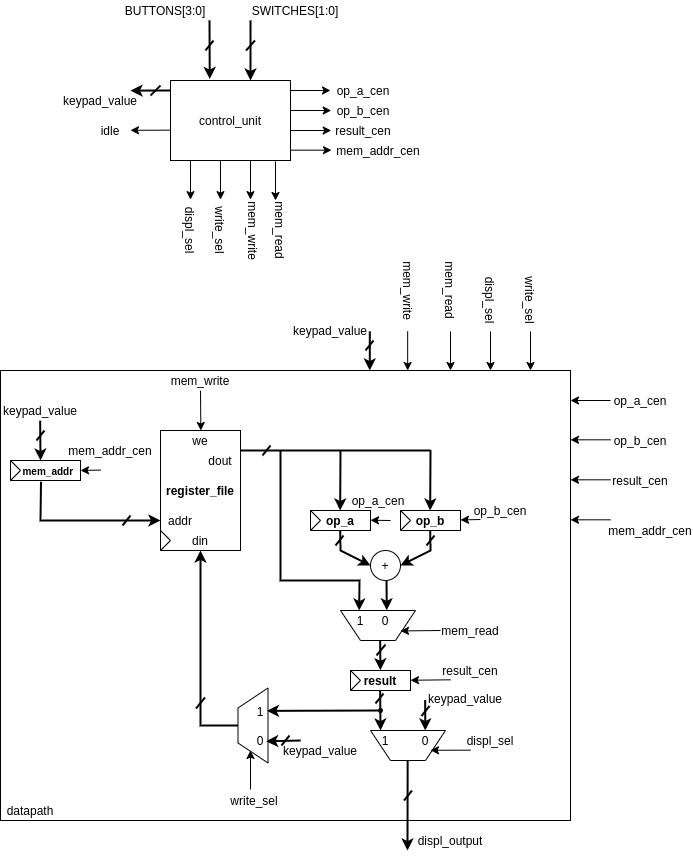
\includegraphics[width=0.7\textwidth]{figs/calculator_datapath_control.png}
\end{center}


Here, the \texttt{keypad\_value} refers to the input value that we set using \texttt{BUTTONS[0]} or \texttt{BUTTONS[1]}. Note how we use a few registers for setting up the address and data input for the register file in the datapath. We also use the registers to prepare the operands for the addition. The datapath module is provided to you. \textbf{Your task is to implement the Control Logic module}. The control logic is in charge of asserting the clock-enable signals for the registers in the datapath, write-enable for the register file, as well as selecting which result to display on the LEDs. Fill in your code in the file \verb|lab3/src/control_unit.v|. Also read the comments in the code for some additional details.

You are also required to use Finite-State Machine (FSM) technique learned from the lectures to implement the calculator. Breaking the functionalities to different states helps you to build the control logic for your calculator more naturally. Initially, your calculator is in an idle state, and you use the switch configuration with \texttt{BUTTONS[3]} to transition to another state, and back to the idle state when a command/task is finished. Before you begin coding, try drawing a FSM diagram of your control logic, and think of when a particular control signal should be asserted.

You are free to make any assumption regarding the functionalities of the calculator in cases where the description above does not cover. Please also feel free to change the datapath module if it makes your design more efficient or functional.

When you are done with implementing your control logic module, write your own testbench to verify your design, then generate a bitstream with \verb|lab3/src/z1top_calculator.v| as the top-level module to test it on your PYNQ board.

Don't hesitate to ask a TA if you need some clarifications for this task.

%\newpage
\section{Lab Deliverables}
\subsection{Lab Checkoff (due: 11.00AM, Feb 17th, 2021)}
To checkoff for this lab, have these things ready to show the TA:
\begin{enumerate}
  \item Demonstrate working accumulation designs with ASYNC\_ROM and SYNC\_ROM.
  \item Demonstrate a working calculator. Your calculator should be able to store data, load data, and add two operands. As an example, try storing the values 2, 4, 6, 8 to the locations 1, 2, 3, 4 of the Register File, respectively. and perform the addition of the data from the location 1 and 2, and store the result to location 5. Next, perform a load at one location to see if data gets written correctly.
\end{enumerate}

\subsection{Lab Report (due: 11.59PM, Feb 17th, 2021)}\label{sec:labreport}
\begin{enumerate}
  \item Your answers to the questions in sections \ref{sec:Q1}, \ref{sec:Q2}, and \ref{sec:Q3}. In addition, please also submit the FSM diagram of your control unit. Be sure to indicate the conditions for all the output control signals. For brevity, you can write Boolean expressions for them instead of drawing logic gates.
\end{enumerate}

\newpage
\section*{Ackowlegement}
This lab is the result of the work of many EECS151/251 GSIs over the years including:
\begin{itemize}
\item Sp12: James Parker, Daiwei Li, Shaoyi Cheng
\item Sp13: Shaoyi Cheng, Vincent Lee
\item Fa14: Simon Scott, Ian Juch
\item Fa15: James Martin
\item Fa16: Vighnesh Iyer
\item Fa17: George Alexandrov, Vighnesh Iyer, Nathan Narevsky
\item Sp18: Arya Reais-Parsi, Taehwan Kim
\item Fa18: Ali Moin, George Alexandrov, Andy Zhou
\item Sp19: Christopher Yarp, Arya Reais-Parsi
\item Fa19: Cem Yalcin, Rebekah Zhao, Ryan Kaveh, Vighnesh Iyer
\item Sp20: Tan Nguyen
\item Fa20: Charles Hong, Kareem Ahmad, Zhenghan Lin

\end{itemize}

\end{document}
